
\chapter{Результаты}\label{chapt_results}
В результате полугода работы прибора ДЭПРОН накоплен большой массив информации - 25 тысяч файлов бинарных данных, общим объемом 100 МБайт. Первичные данные были распакованы и сохранены в текстовом виде.
Далее информация прибора ДЭПРОН была визуализирована с помошью пакета \texttt{lattice} и базовой графической системы R. 
В первую очередь для каждого дня работы прибора были построены карты скоростей счета в детекторе 1\ref{sec:planetDose}.В процессе построения пространственного распределения было обнаружено расхождение меток времени  ДЭПРОН и всемирного времени. Разработанное решение проблемы привязки данных подробно рассматривается в разделе \ref{sec3.2}.

Аналогично картам были построены долготные зависимости скоростей счета в первом детекторе, эти графики позволили оперативно заметить резкие всплески потоков частиц во внешнем радиационном поясе. Также для каждого дня были построены карты скоростей счета в координатах Мак-Илвайна, рассчитанным по модели IGRF.

\section{Планетарное распределение потоков частиц, мощности дозы на высоте полета КА а также потоков нейтронов} \label{sec:planetDose}
При последующей обработке данных были построены графики географического распределения скоростей счета во всех детекторах прибора - двух полупроводниковых и двух нейтронных счетчиков. Цветовая схема для карт подобрана таким образом, чтобы максимальные значения были отображены красным цветом а минимальные синим, между конечными точками цвет изменяется по градиенту. Цветовая палитра квантизована на 20 дискретных цветов. Каждому значению полученной дозы ставится в соответствие индекс в массиве цветов, который вычисляется по формуле:

\[ i_{color}  = \left\lbrace{8*\log{10}(I) + 1} +1, если 8*\log{10}(I) + 1} +1<n;
							n, если 8*\log{10}(I) + 1} +1>=n\]
						
						
% col = colr[ifelse(ceiling(8*log10(as.integer(combined.zoom$count1)+1))+1>n,
%n,
%ceiling(8*log10(as.integer(combined.zoom$count1)+1))+1)]
%
На картах каждый маркер представляет результаты измерений детекторов за одну секунду. В качестве маркера выбран незакрашенный круг, так как в отличие от точки или линии он позволяет покрыть некоторую площадь на графике. Размер маркера подобран исходя из соображений заметания определенной площади, так как  при полете по орбите спутник покрывает 7,5 км каждую секунду. Маркеры частично перекрываются, особенно в полярных областях и наилучшие результаты по отображению были получены при использовании частичной прозрачности. Для простоты отображения выбрана прямоугольная проекция карты по широте и долготе, поэтому на различных широтах площадь отображаемой поверхности не искажена. Это обстоятельство таким образом лишь условно соответсвует величине траектории вдоль которой производилось измерение.

\section{Распределения мощности дозы в области ЮАА}
Временные серии скоростей счета и мошьности дозы, полученные с Дэпрон для 14:30 29 Августа 2016 года. Возрастание скоростей счета и доз связано с пересечением ЮАА. Точками показаны измерения с детекторов с секундным разрешением, сплошными линиями отражено сглаживание данных треугольным фильтром.
\begin{figure}
	\centering
	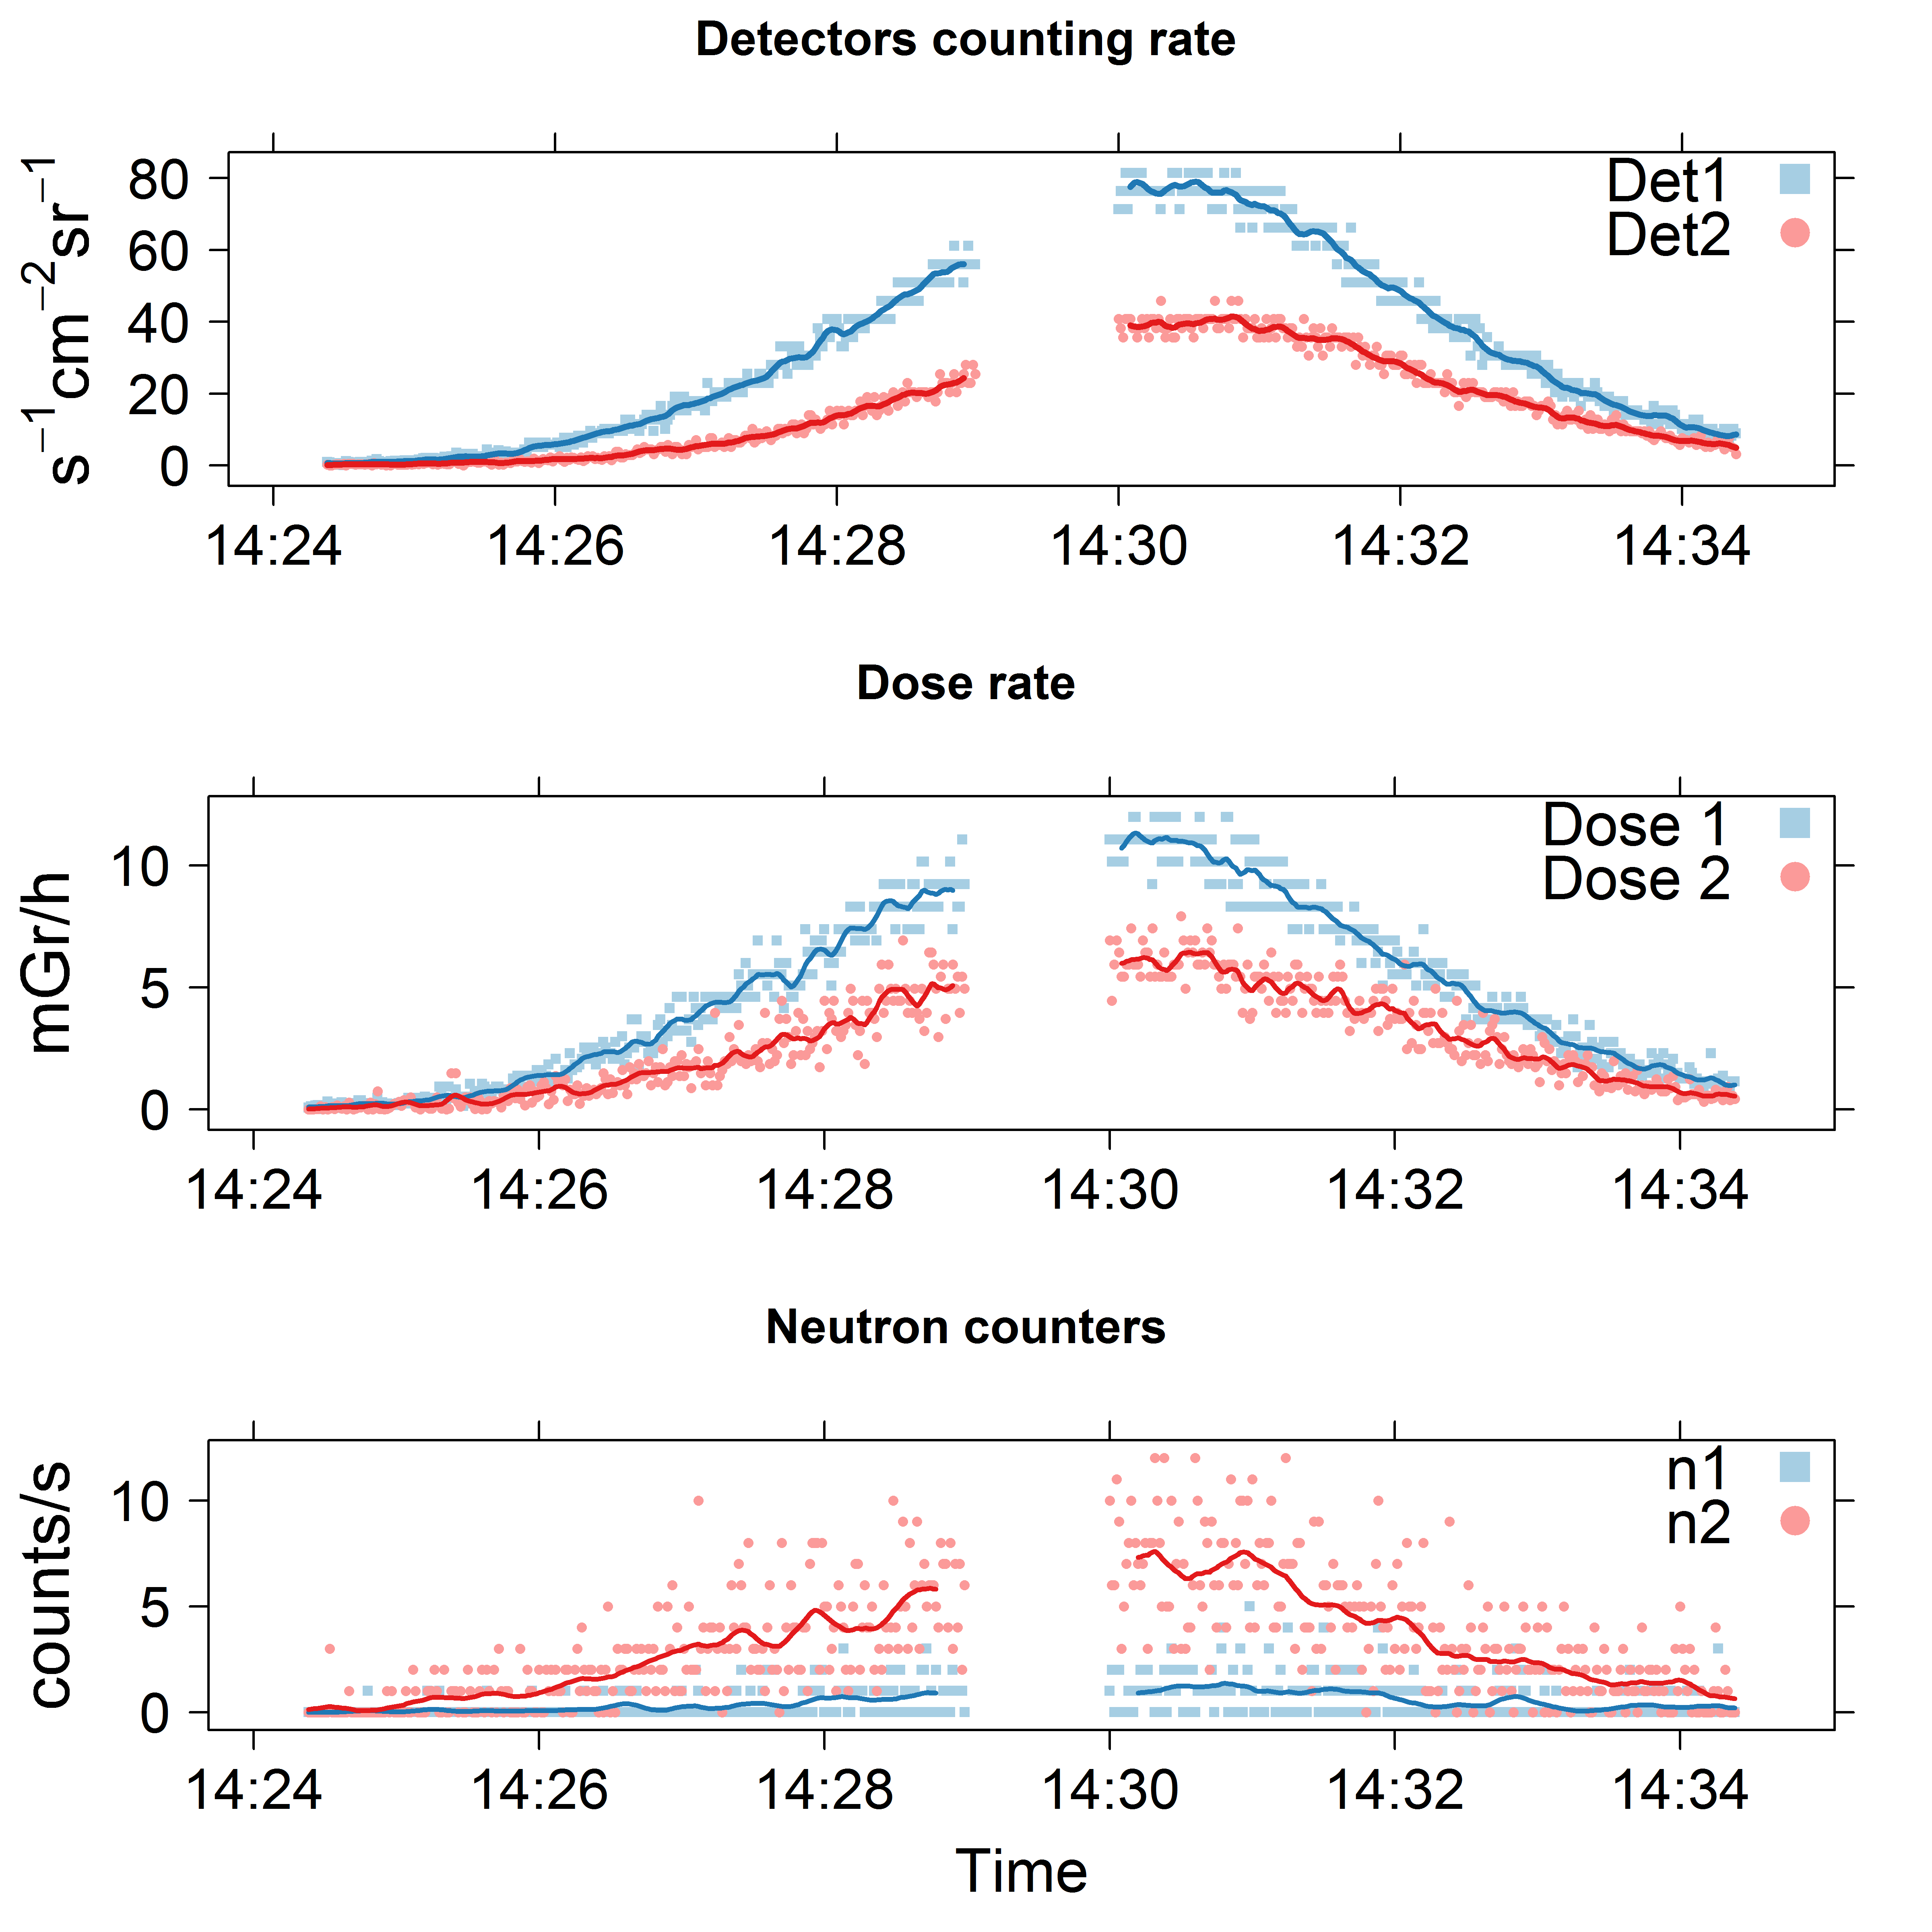
\includegraphics[width=0.7\linewidth]{images/results/depron_sec_log_new08-29-1614-24-23}
	\caption{Временные серии скоростей счета и мошьности дозы при пересечении внутреннего радиационного пояса}	\label{fig:depronseclognew08-29-1614-24-23}
\end{figure}


\section{Распределения мощности дозы в авроральных областях}
Приполярные области отличаются высокой вариабельностью потоков частиц и соответственно доз. В основном повышенные потоки регистрируются в первом полупроводниковом детекторе, что говорит о невысоких энергиях частиц в этих потоках.

\begin{figure}[h]
	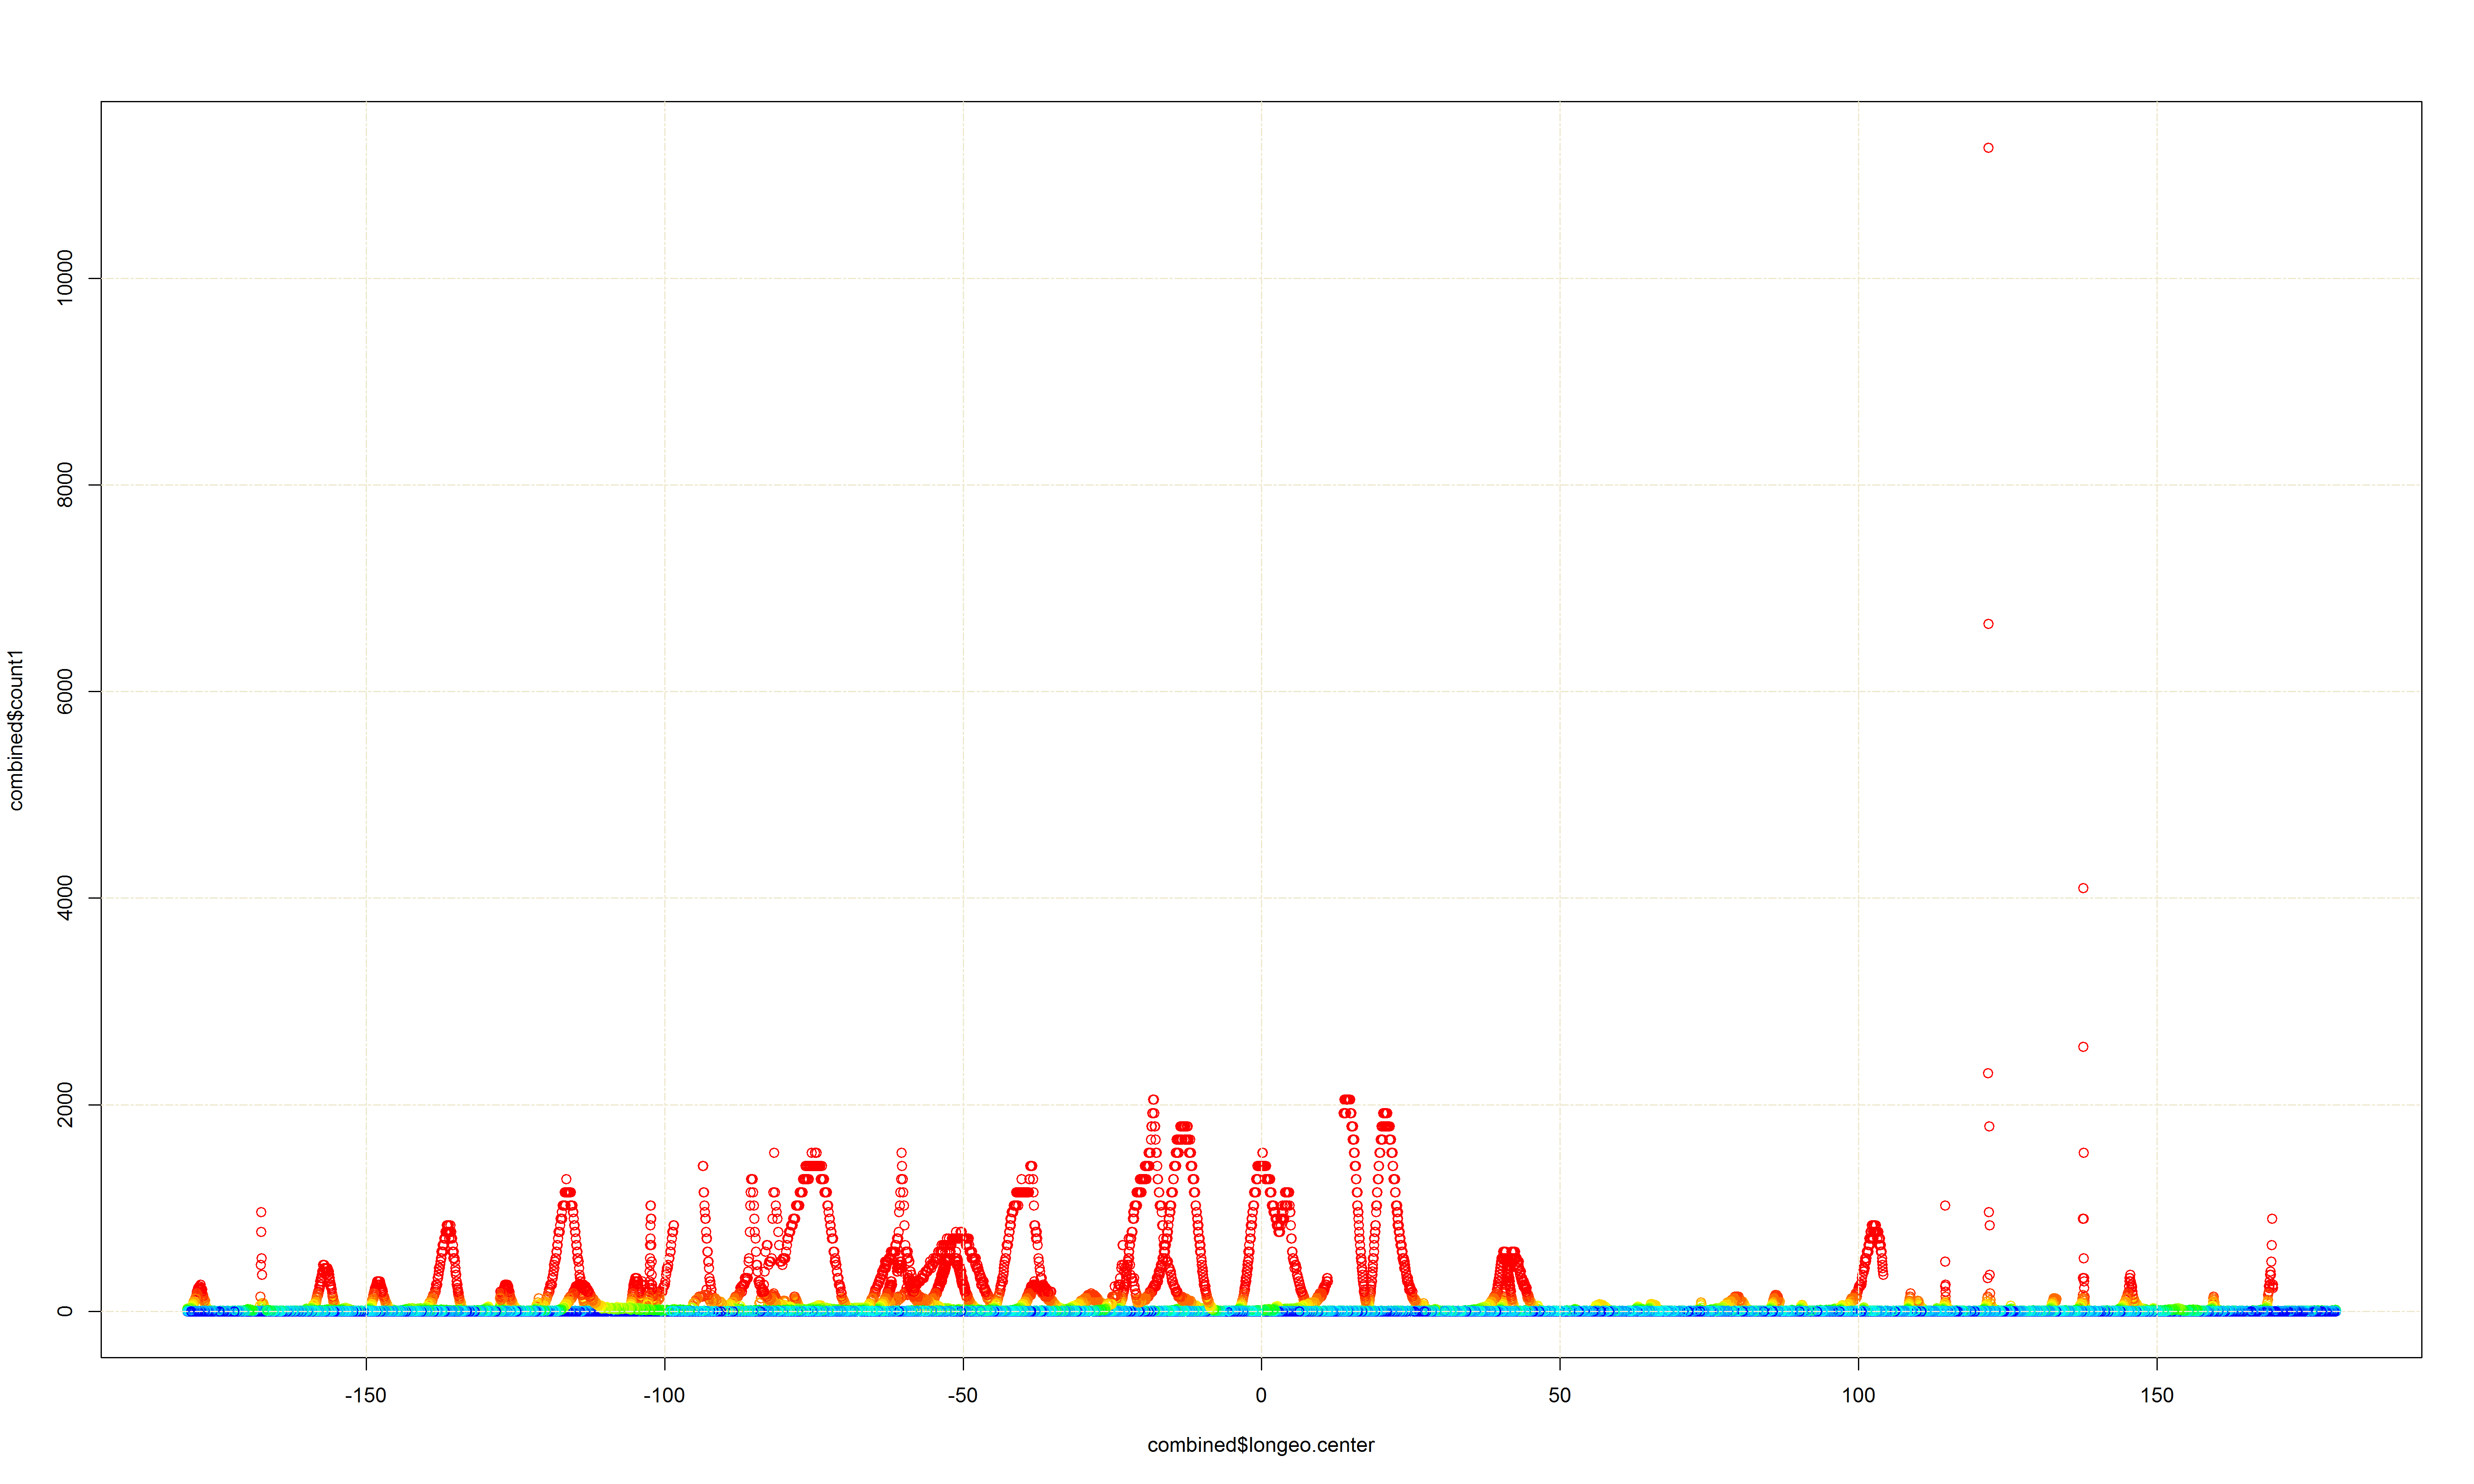
\includegraphics[width=0.8\linewidth]{images/Flash/depron_lat_map_148}
	\caption{Географическое распределение потоков заряженных частиц в первом полупроводниковом детекторе}
	\label{fig:depronlatmap148}
\end{figure}
Рассмотреть зависимости дозы в L-B координатах разделив при этом утреннее в вечернее местное магнитное время (MLT) о наличии магнитной бури следить по индексам A(e) A(l), причем по мнению Антоновой стоит выбрать спокойный период.

Построены зависимости B(t) для L из диапазонов от 4-5, 5-6, 6-7.

\begin{figure}
	\centering
	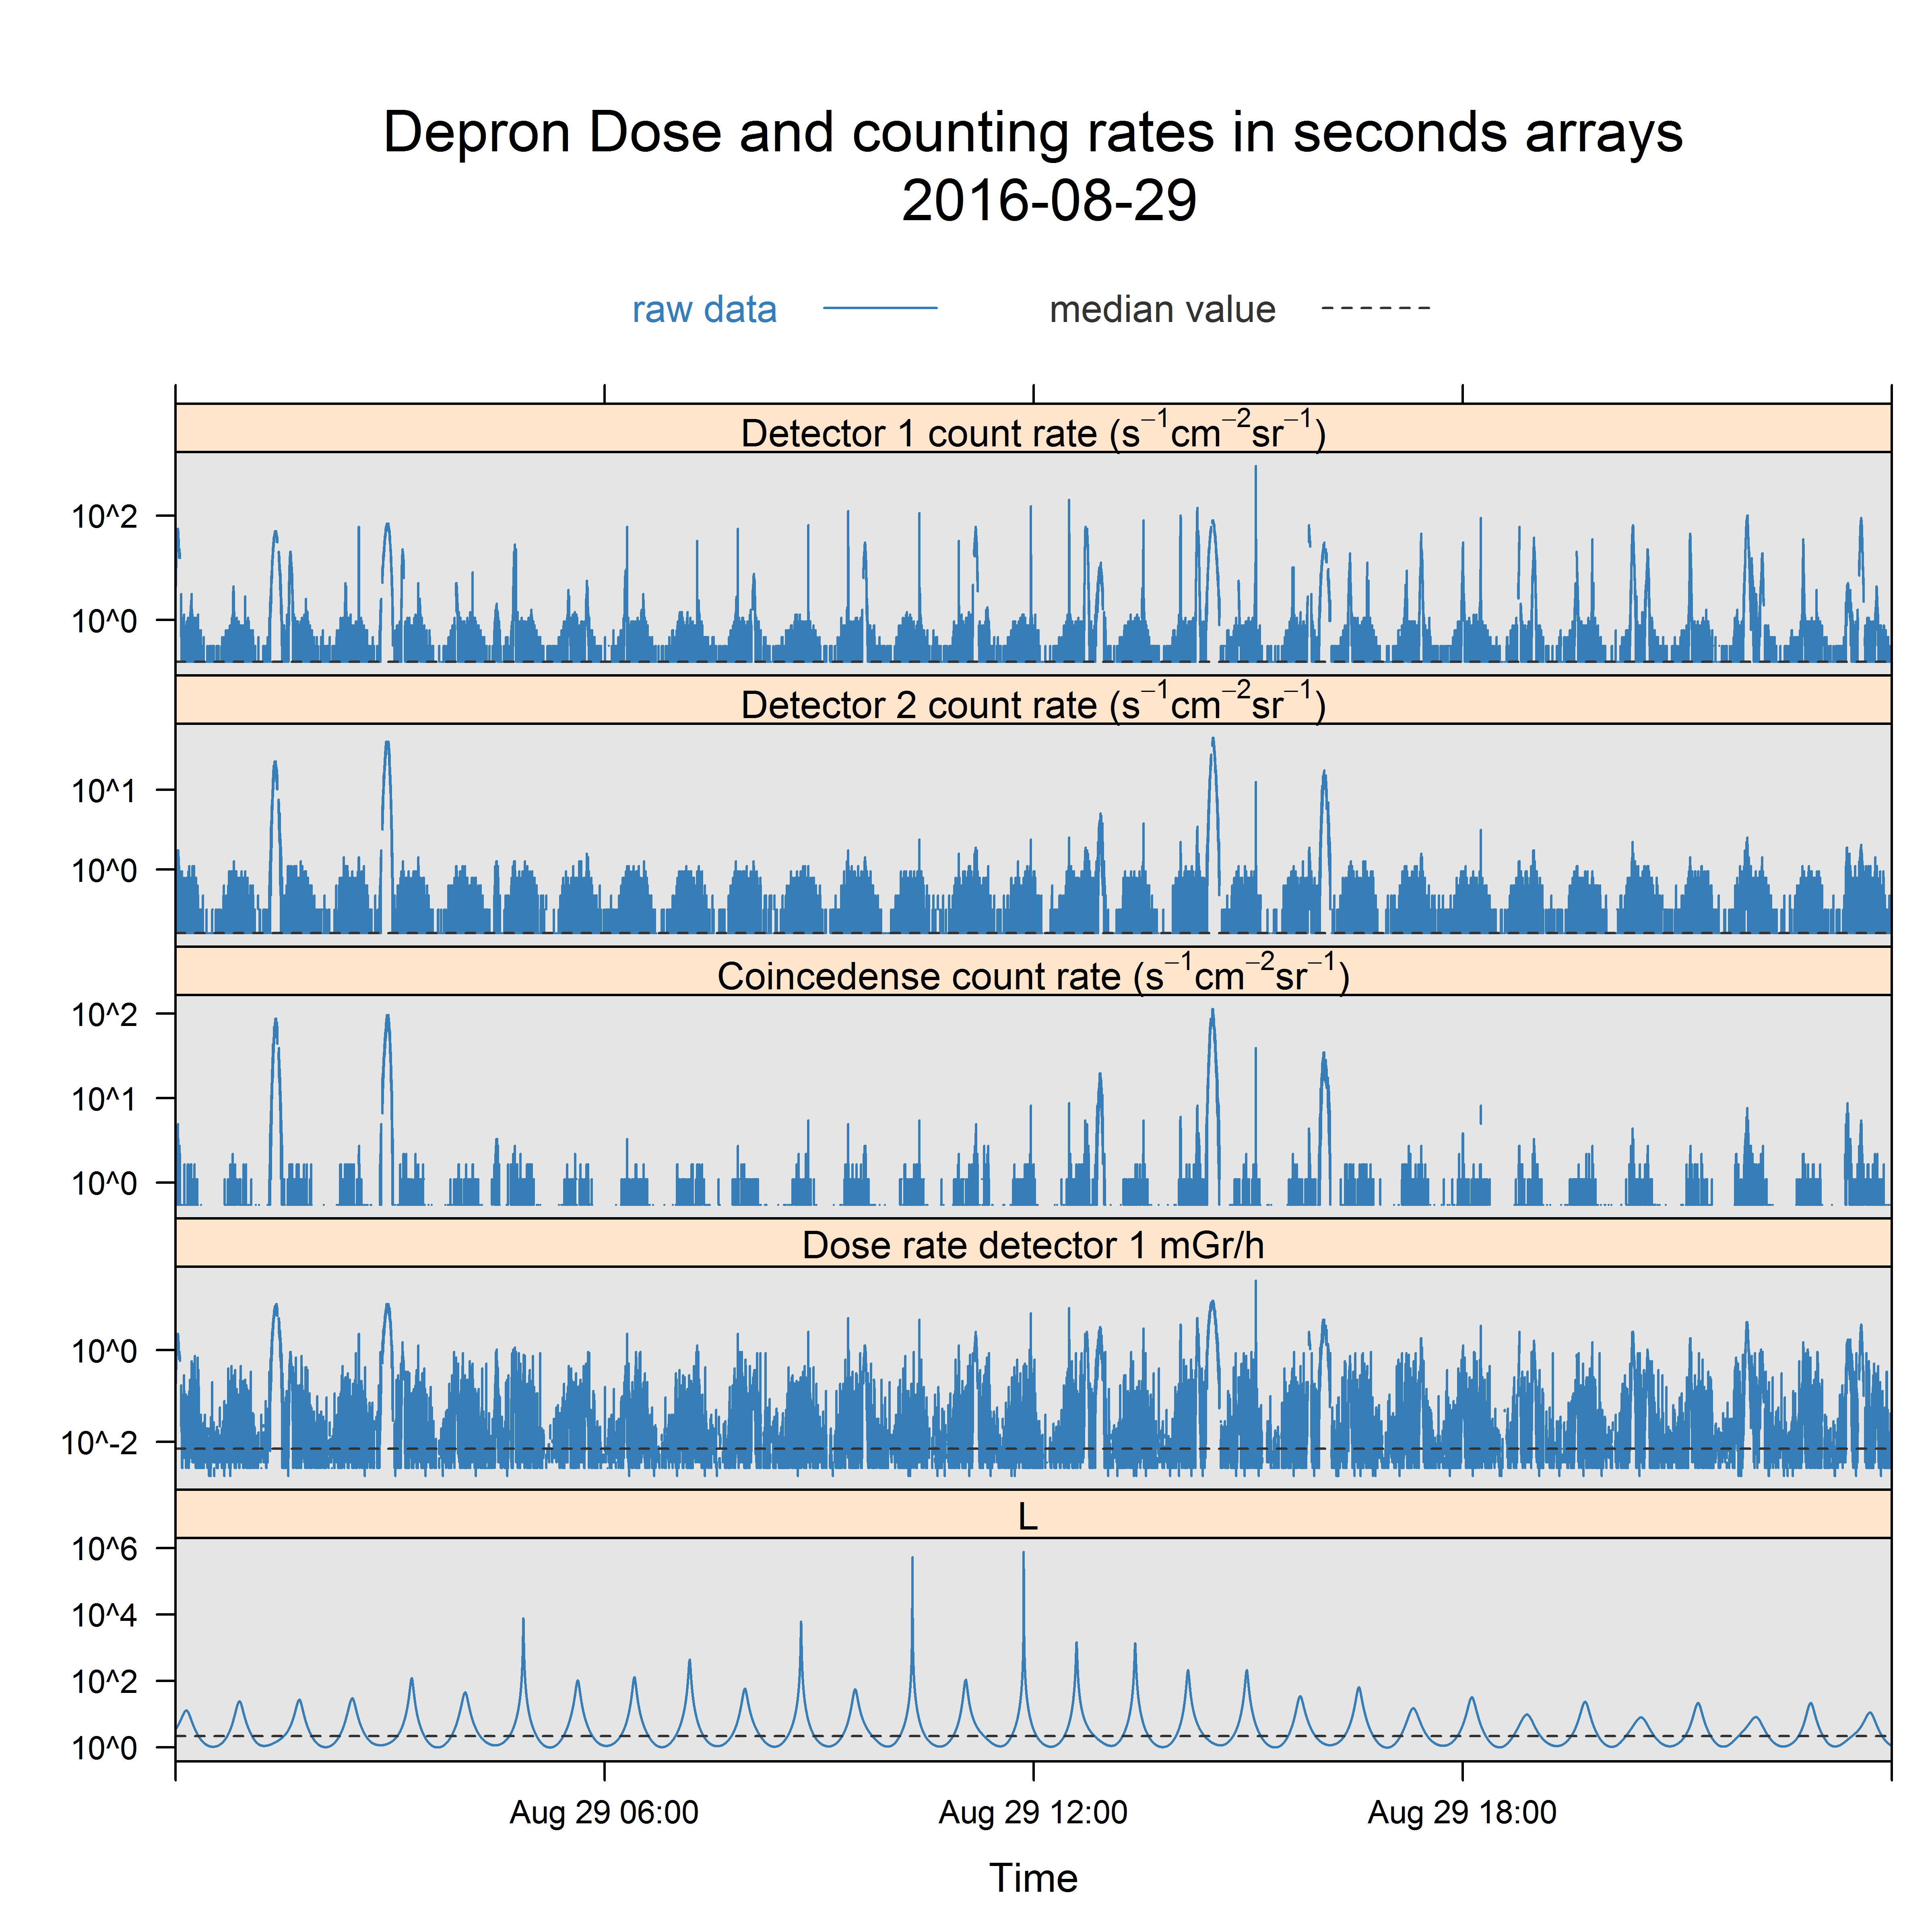
\includegraphics[width=0.7\linewidth]{images/results/depron_sec_log08-29-16}
	\caption{Временные серии в детекторах прибора.}
	\label{fig:depronseclog08-29-16}
\end{figure}
На рисунке \ref{fig:depronseclog08-29-16} показаны 
\begin{figure}
	\centering
	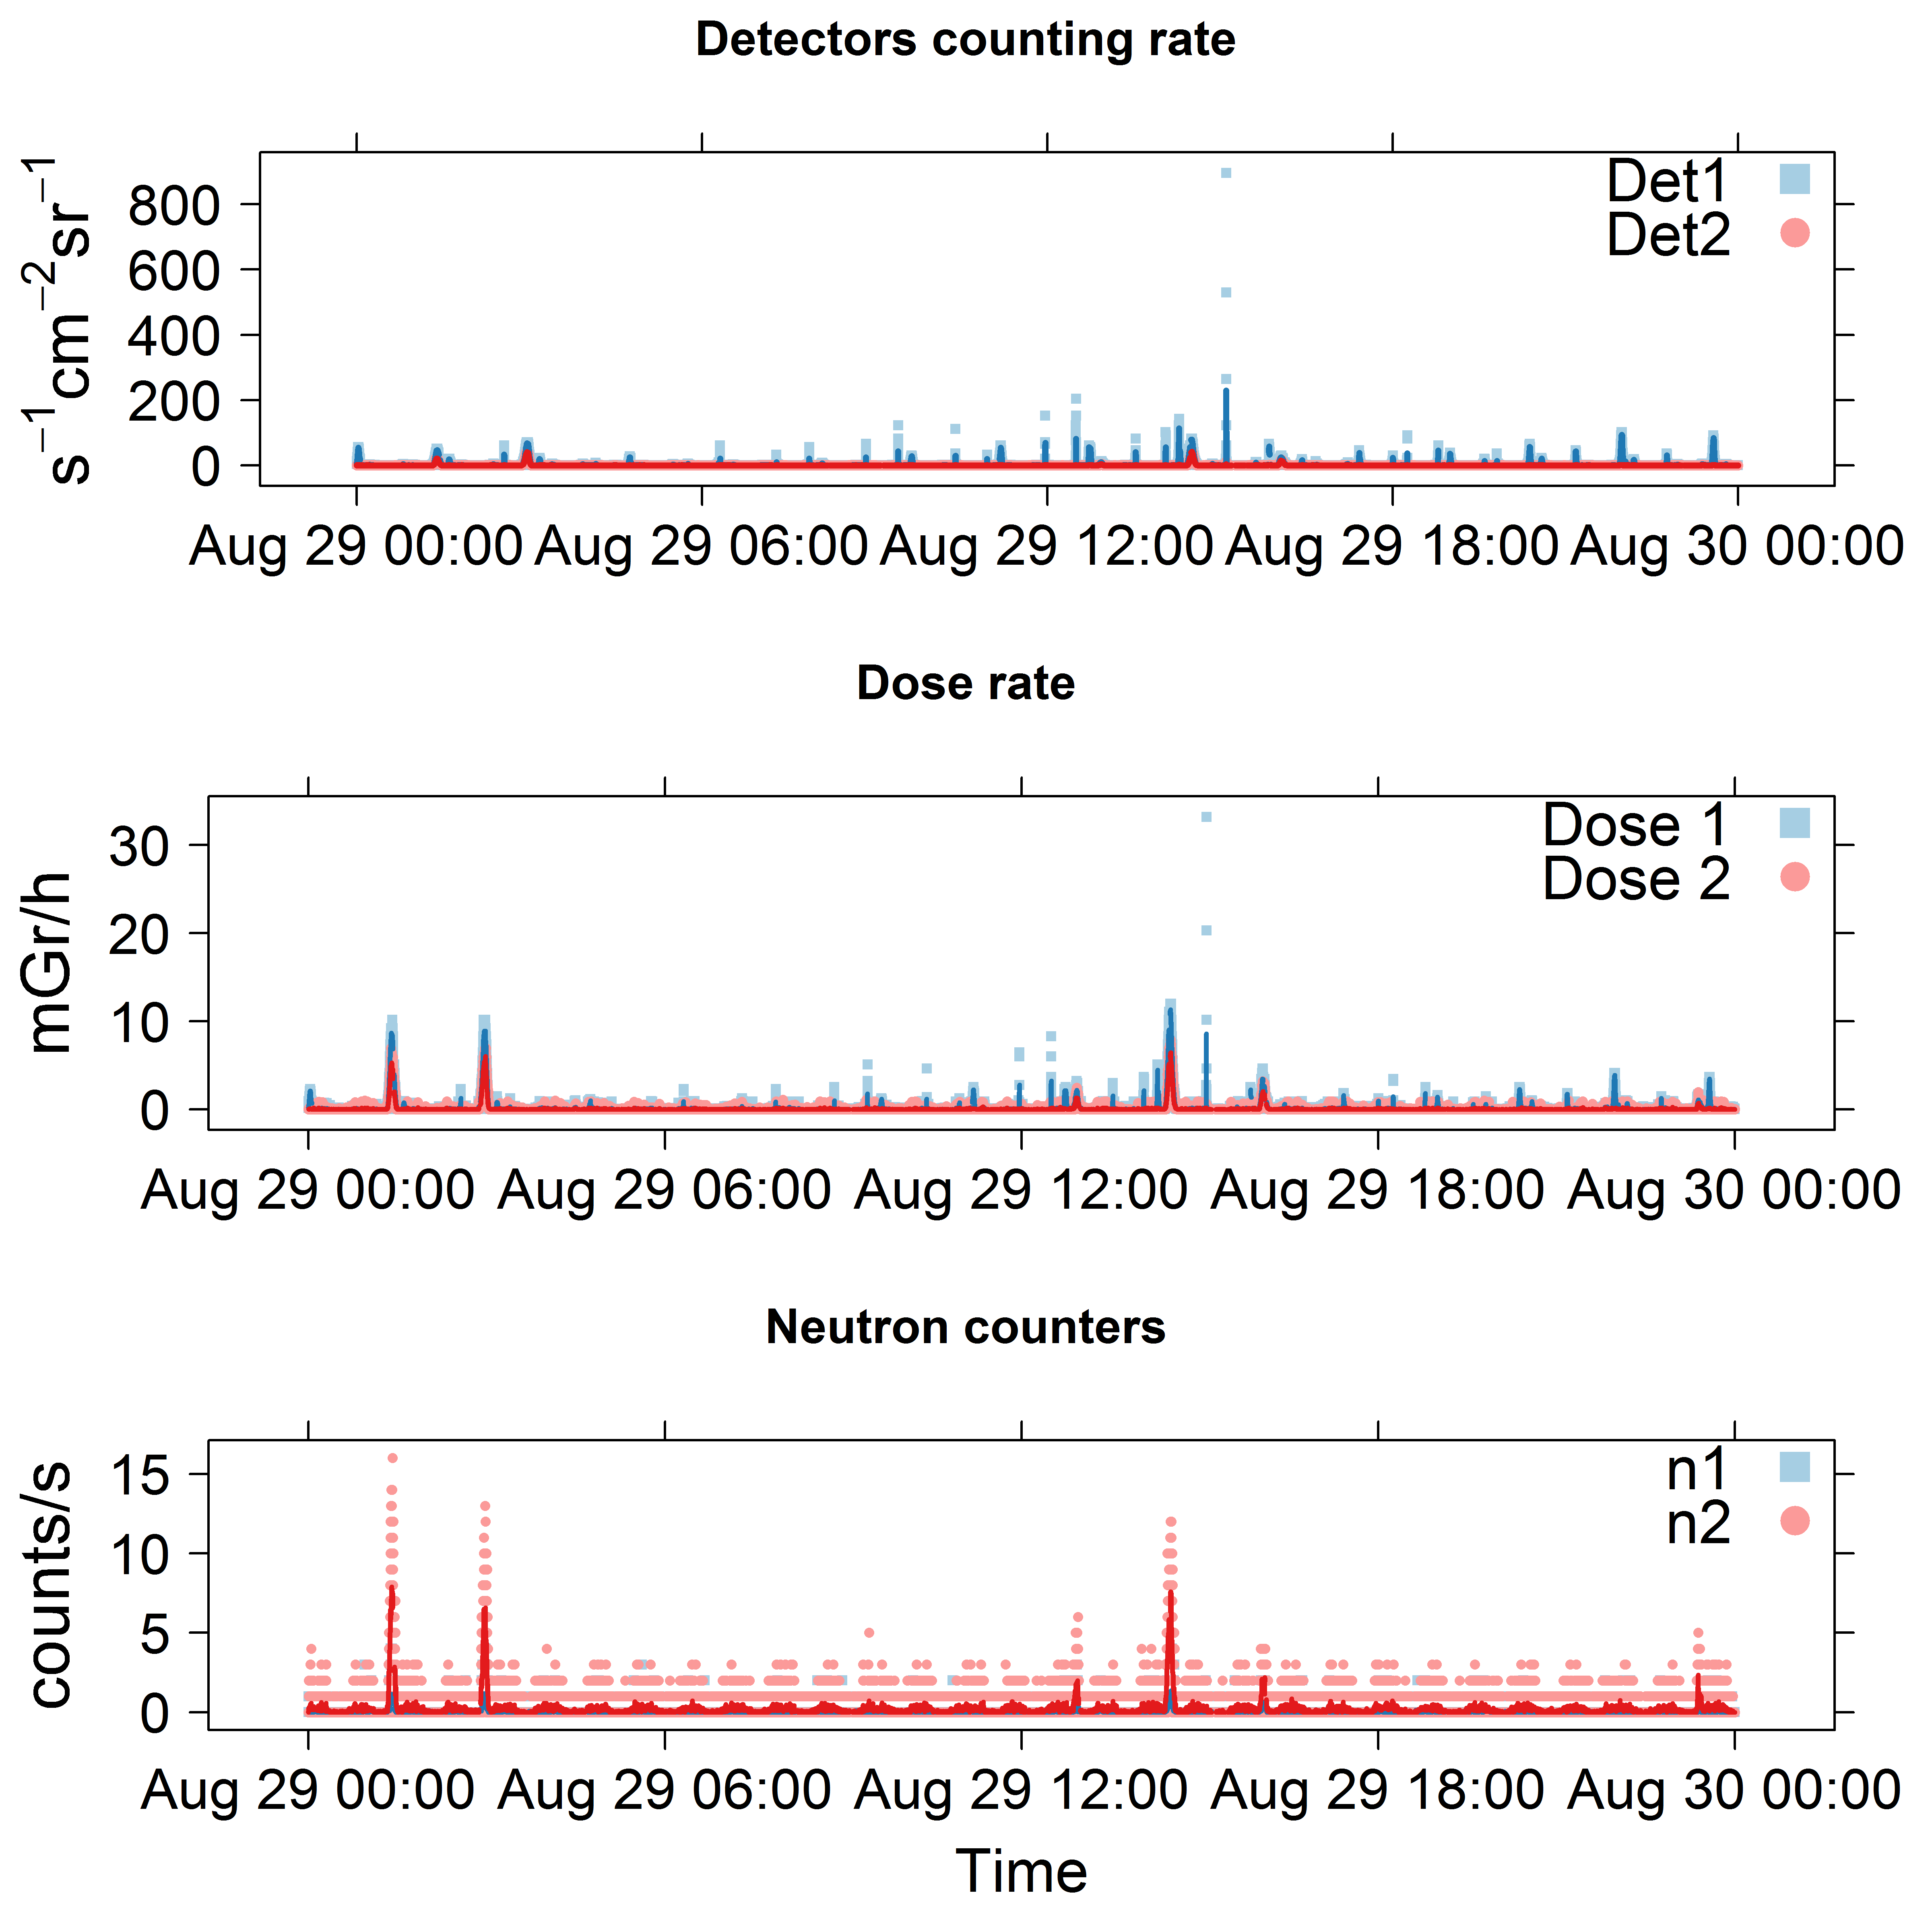
\includegraphics[width=0.7\linewidth]{images/results/depron_sec_log_new08-29-16}
	\caption{}
	\label{fig:depronseclognew08-29-16}
\end{figure}
Счет в детекторах прибора  

\begin{figure}
	\centering
	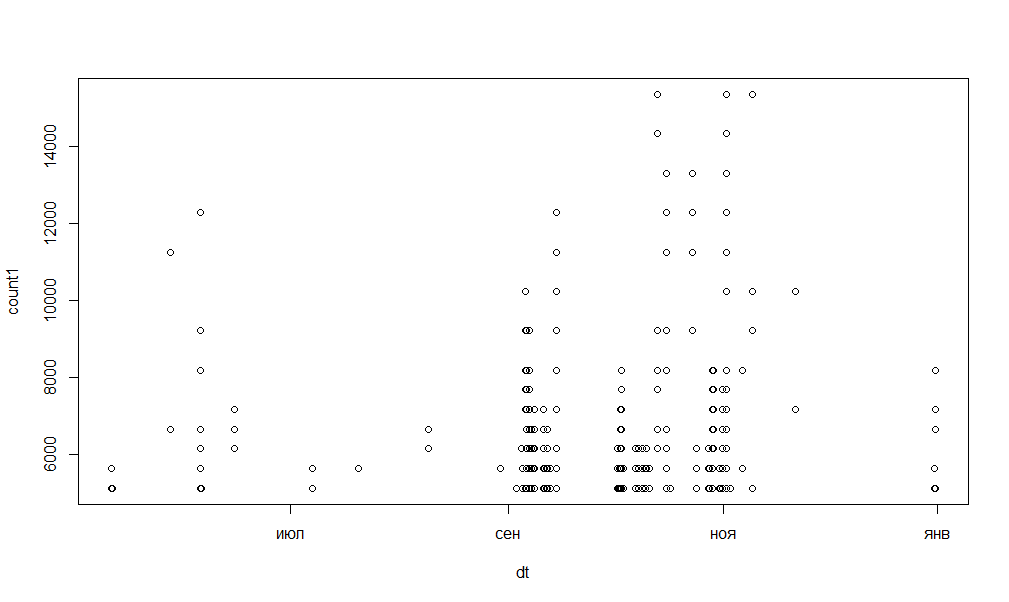
\includegraphics[width=0.7\linewidth]{images/Flash/Rplot03}
	\caption{}
	\label{fig:rplot03}
\end{figure}

\begin{figure}
	\centering
	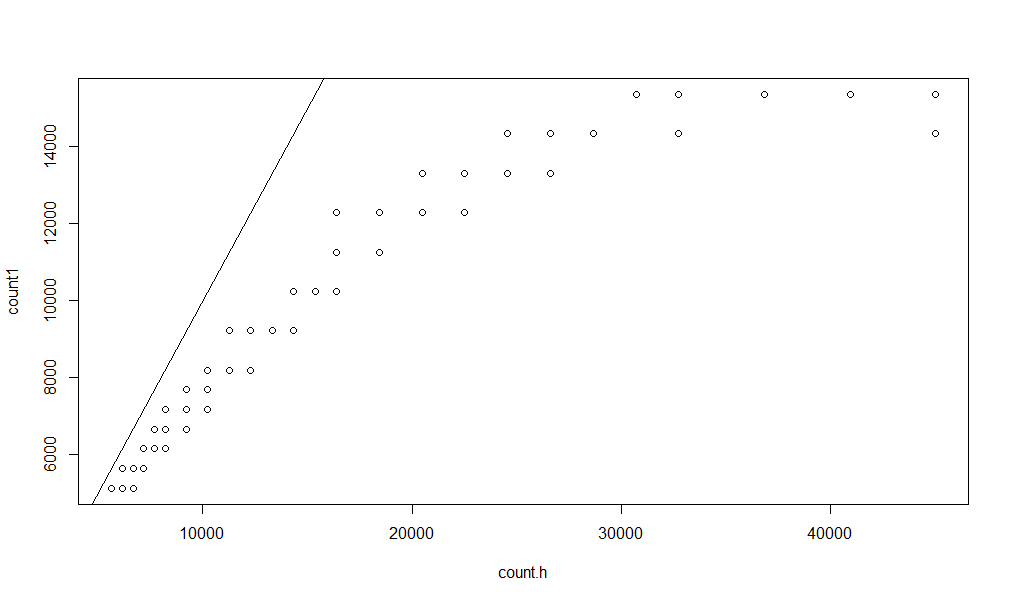
\includegraphics[width=0.7\linewidth]{images/Flash/Rplot04}
	\caption{}
	\label{fig:rplot04}
\end{figure}



\begin{figure}
	\centering
	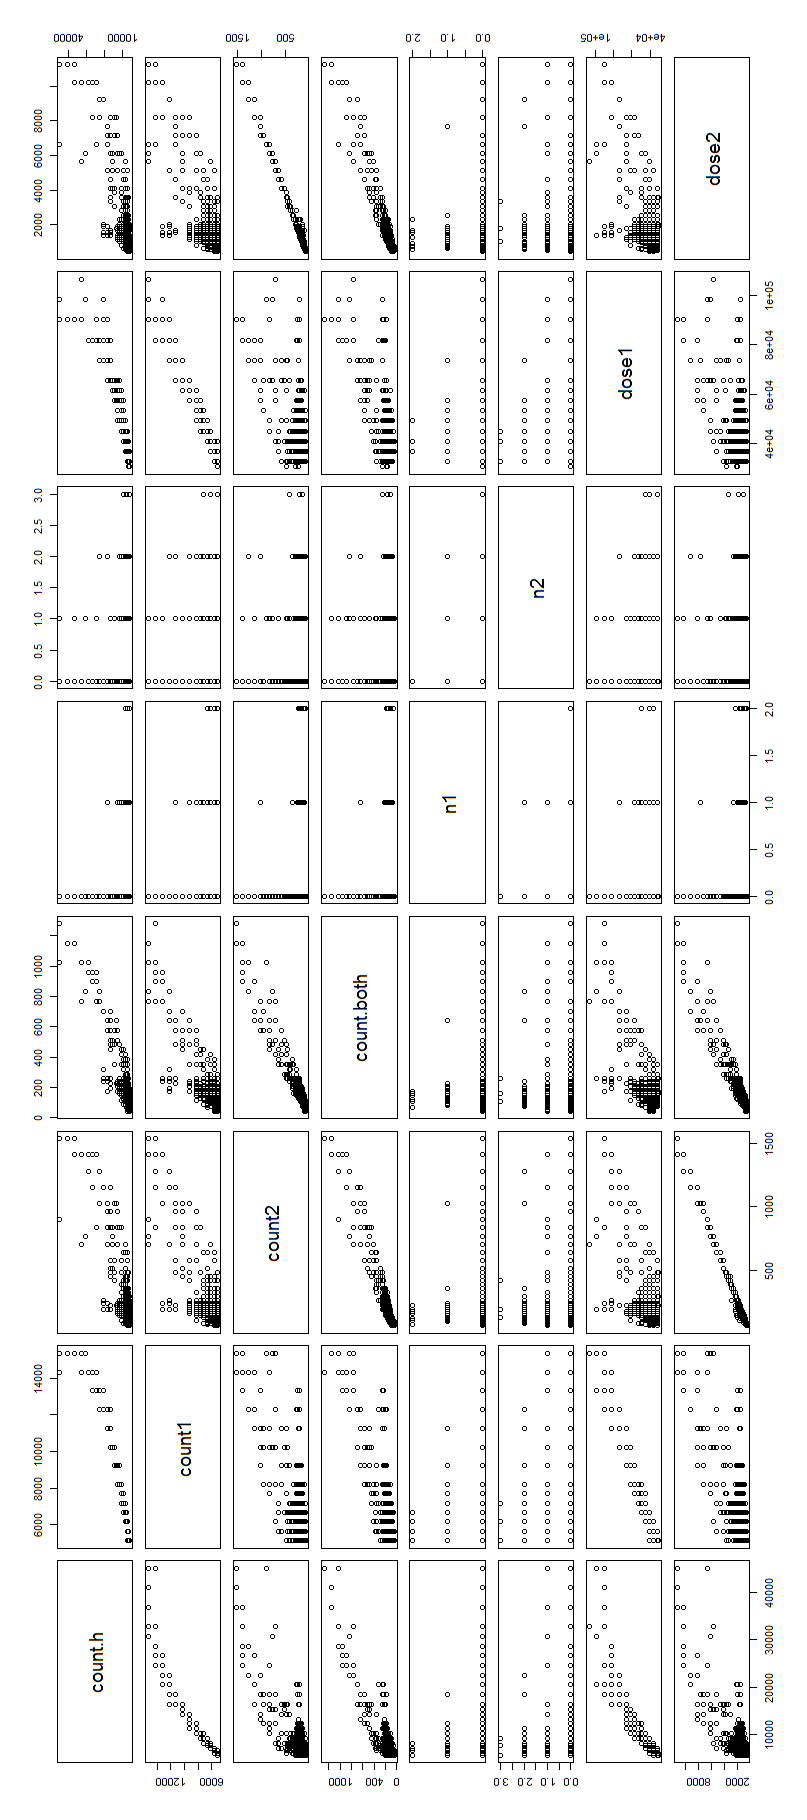
\includegraphics[width=0.7\linewidth]{images/Flash/Rplot06}
	\caption{}
	\label{fig:rplot06}
\end{figure}

\begin{figure}
	\centering
	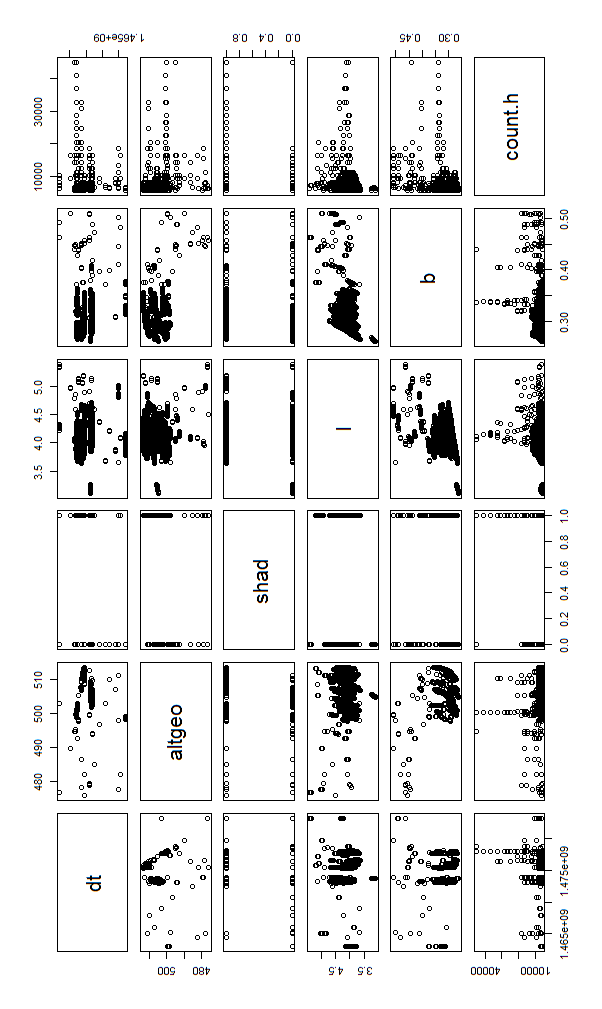
\includegraphics[width=0.7\linewidth]{images/Flash/Rplot08}
	\caption{}
	\label{fig:rplot08}
\end{figure}

\section{Распределение мощности дозы вне радиационных поясов Земли}

\section{Спектры ЛПЭ и распределение мощности эквивалентной дозы}